In ASCETIC la persistenza dei dati è necessaria soprattutto per tenere traccia di informazioni importanti ai fini delle funzioni offerte dal sistema. ASCETIC infatti deve essere in grado di: memorizzare le informazioni temporali relative all'ultima modifica del progetto, ricordare la struttura di quest'ultimo, ossia memorizzare quali e quanti smell vi sono all'interno. Queste caratteristiche rendono più semplice ed immediato il chaching che il sistema sfrutta per mantenere un certo standard in materia di performance. La principale Data Source di ASCETIC è costituita dunque dal codice sorgente del programma preso in esame su IntelliJ: il sistema non sfrutta quindi un vero e proprio DBMS, nonostante l'utilizzo di SQLite (scelto per motivi di ottimizzazione implementativa), ma associa ad ogni progetto un file contenente le informazioni di cui sopra. Lo schema di seguito riportato non costituisce un diagramma ER, bensì uno schema logico rappresentativo del come i file verranno strutturati mediante SQLite.

\hspace{1cm}

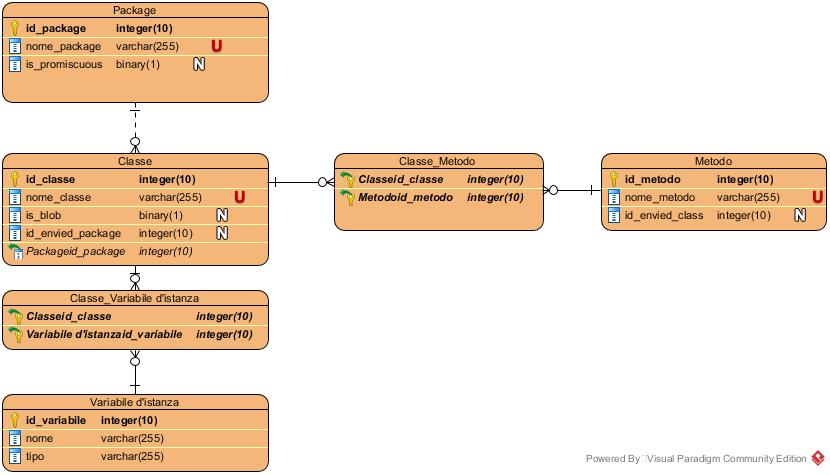
\includegraphics[width=1\textwidth]{Various/schema_logico.jpg}